% Charlotte Geiger - Manuel Lippert - Leonard Schatt
% Physikalisches Praktikum

% 3.Kapitel  Protokoll

% Variables
\def\skalierung{0.65}

\chapter{Messprotokoll}
\label{chap:protokoll}

Das Messprotokoll wurde am Versuchstag handschriftlich erstellt und hier als
PDF-Datei eingefügt.
\section*{Nachtrag}
\begin{itemize}
    \item Fehler der Waage: $u_a=0.05$ kg
    \item Fehler Stoppuhr: $u_t=0.01$ s
\end{itemize}

% Einbindung des Protokolls als pdf (mit Seitenzahl etc.)
% Erste Seite mit Überschrift
%\includepdf[pages = 1, landscape = false, nup = 1x1, scale = \skalierung , pagecommand={\thispagestyle{empty}\chapter{Protokoll}}]
%            {03-Protokoll/Protokoll_KRE.pdf}
% Restliche Seiten richtig skaliert
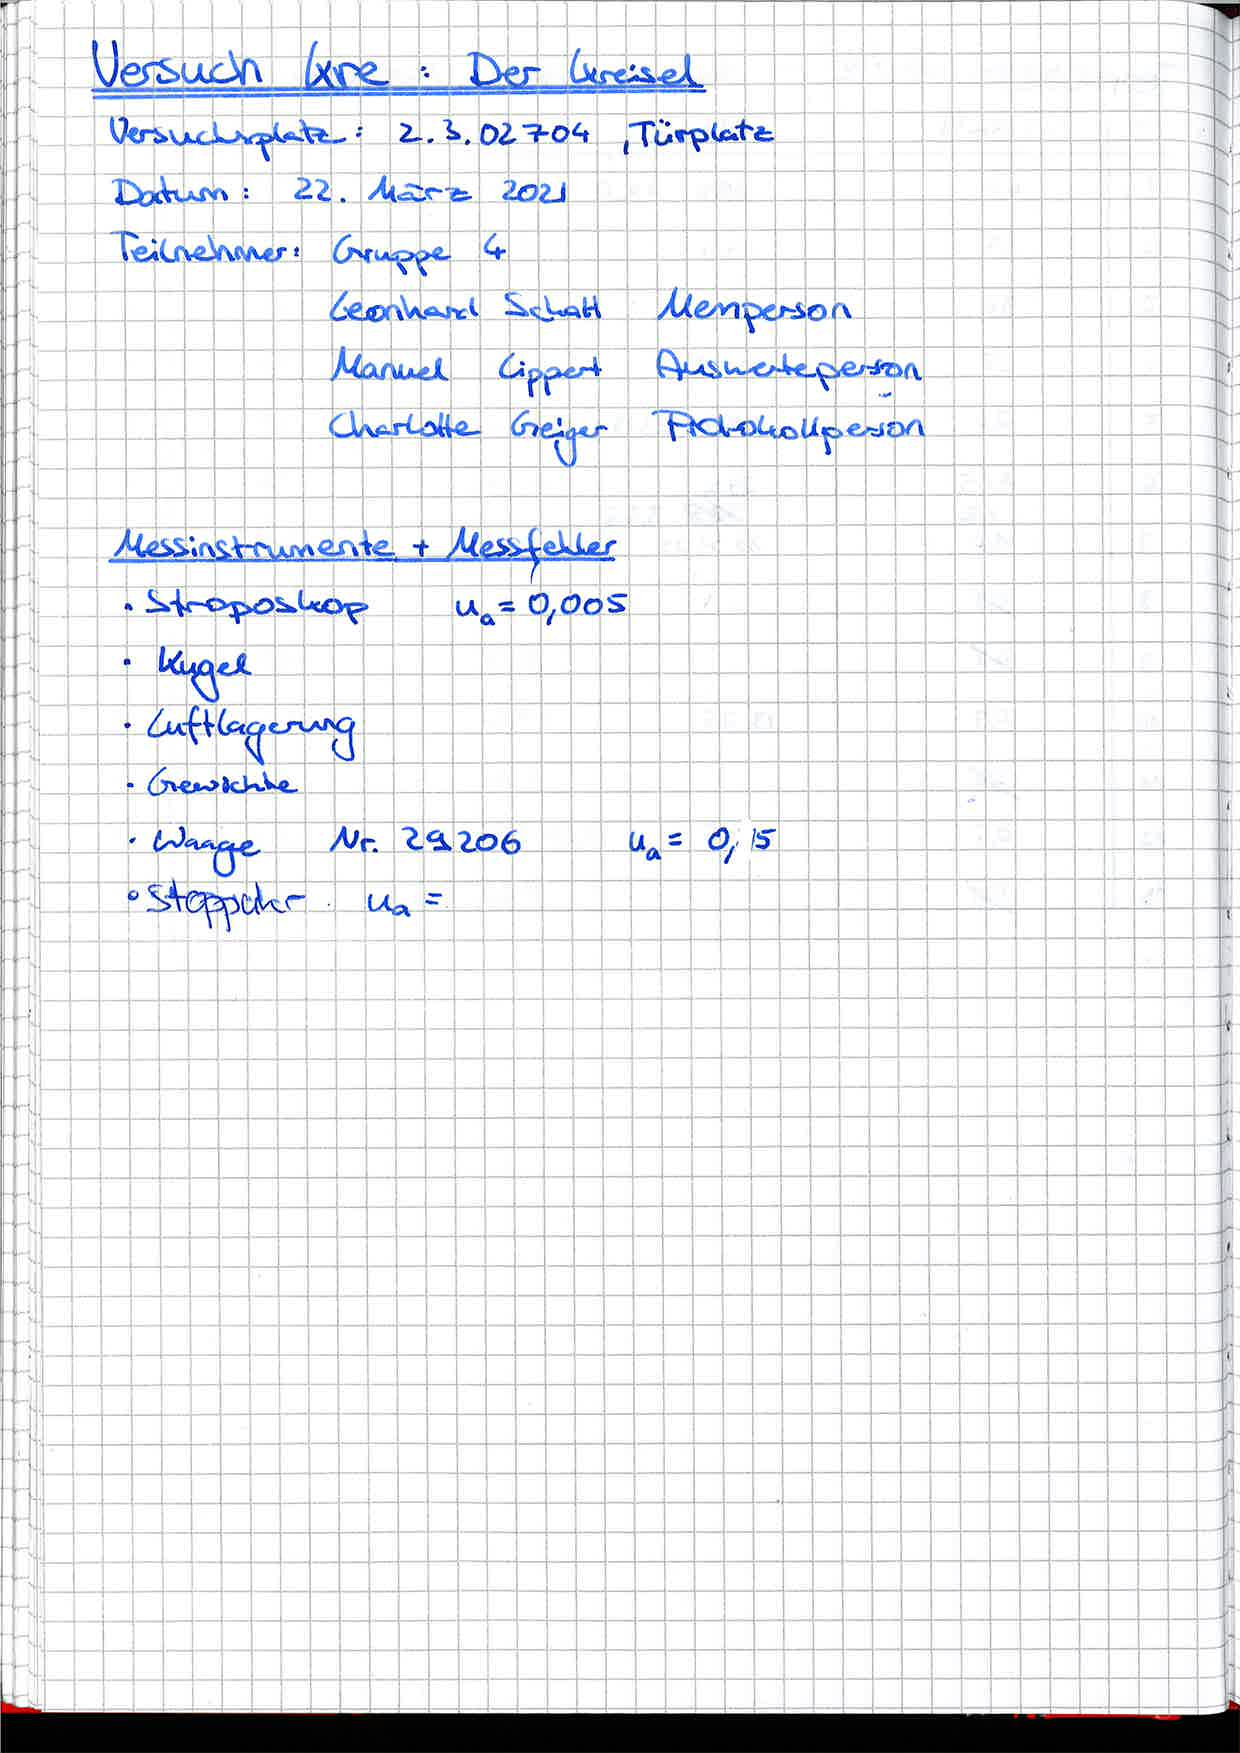
\includepdf[pages = -9, landscape = false, nup = 1x1, scale = \skalierung , pagecommand={}]
            {03-Protokoll/ProtokollKRE.pdf}

\begin{center}
    \begin{tabular}{c c}
        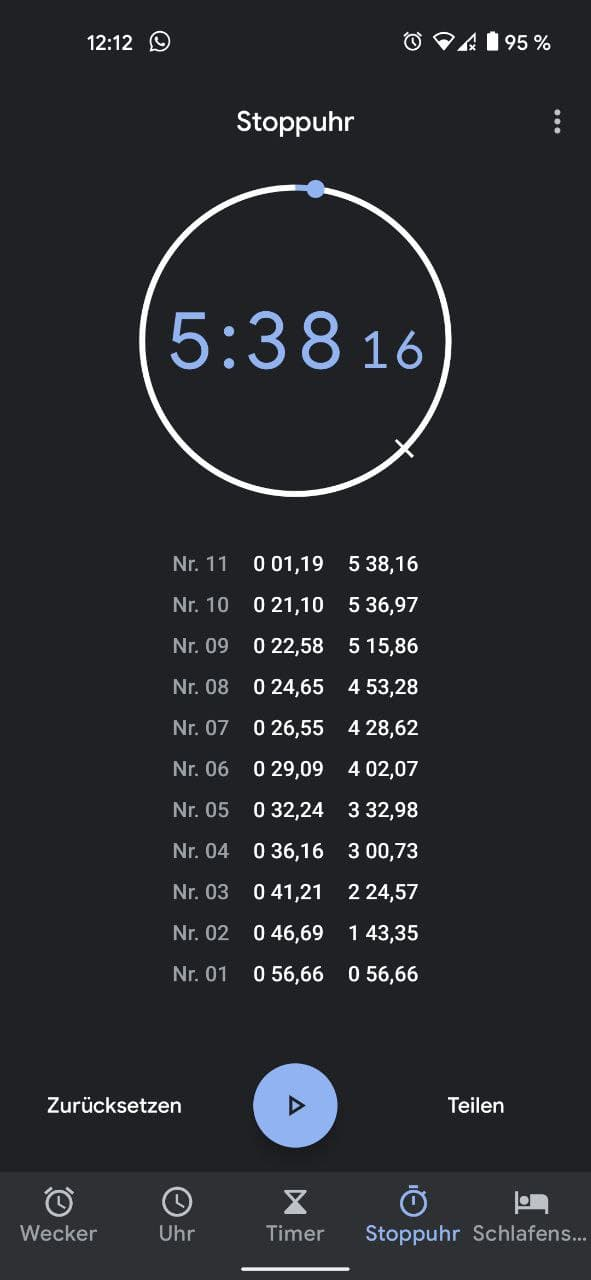
\includegraphics[scale=0.21]{6_3_Screenshots/6_3_Messung1.jpg} \hspace{0.5cm} & \hspace{0.5cm} 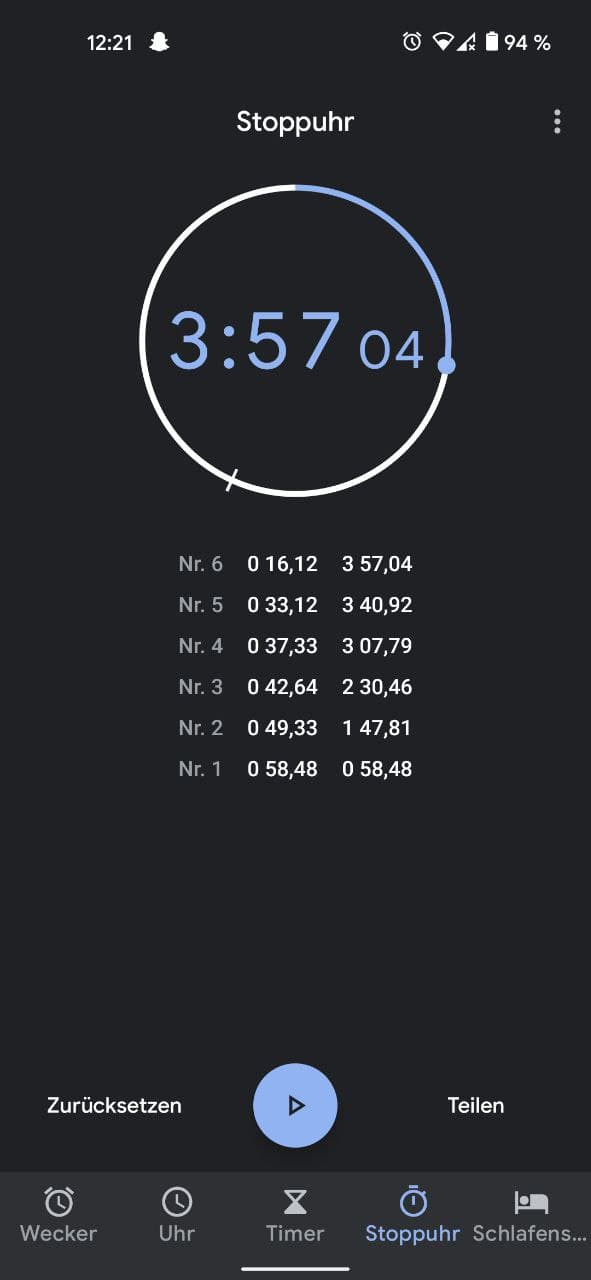
\includegraphics[scale=0.21]{6_3_Screenshots/6_3_Messung2.jpg}\\[0.5cm]            
        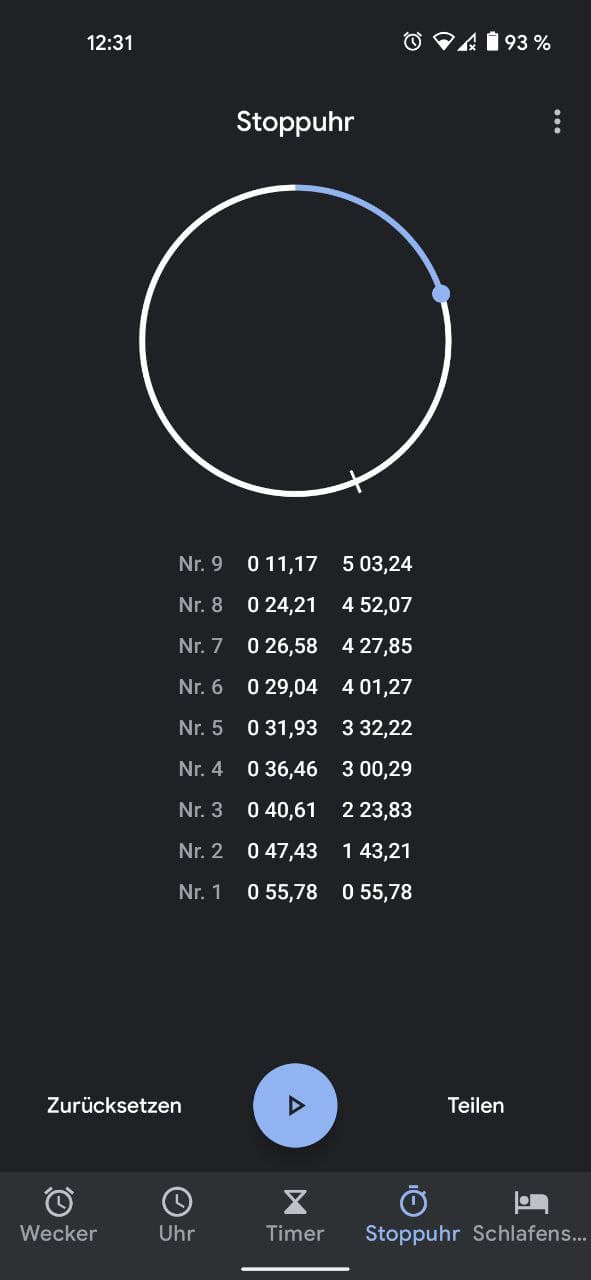
\includegraphics[scale=0.21]{6_3_Screenshots/6_3_Messung3.jpg} \hspace{0.5cm} & \hspace{0.5cm} 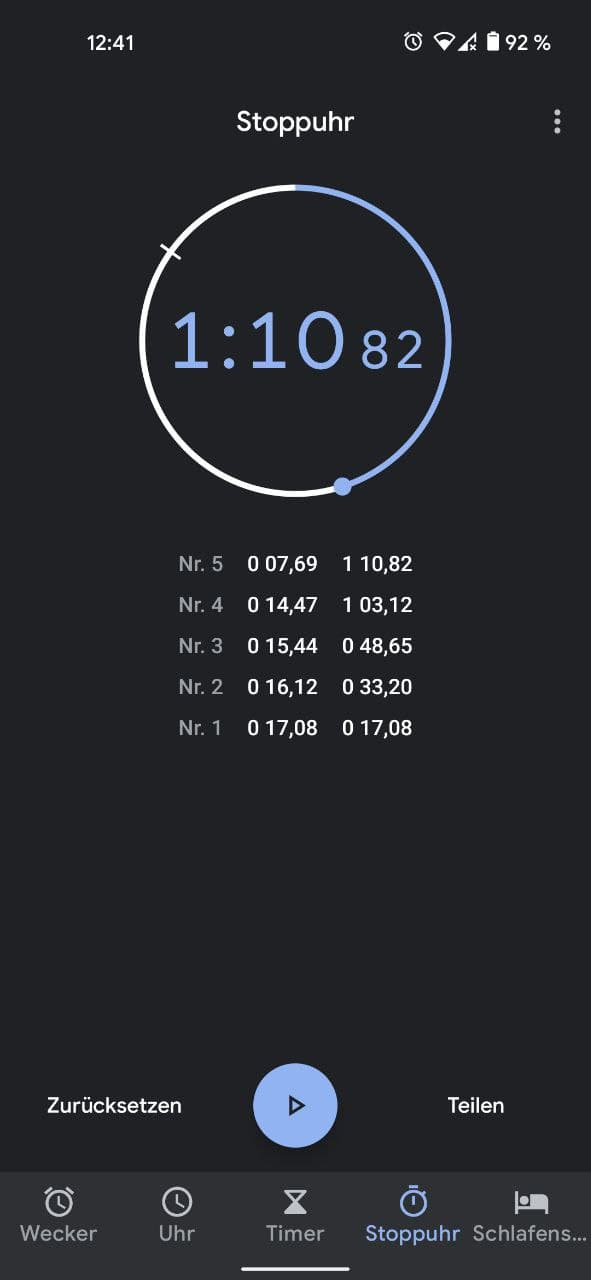
\includegraphics[scale=0.21]{6_3_Screenshots/6_3_Messung4.jpg}            
    \end{tabular}
    \captionof{figure}{Zu Präzession: Messung 1, 2, 3, 4}
\end{center}